% Formatvorlage f�r studentische Arbeiten der Arbeitsgruppe Software Systems
% Engineering am Institut f�r Informatik der Universit�t Hildesheim
%   erstellt von Christopher Voges, 28.04.2016
%   https://sse.uni-hildesheim.de/studium-lehre/richtlinien-fuer-ausarbeitungen/vorlagen/

% Dokumentenkopf 
\documentclass[
    11pt, % Schriftgr��e
    DIV=10,
    a4paper, % Papierformat
    twoside, % einseitiges Dokument
    titlepage, % es wird eine Titelseite verwendet
    parskip=half, % Abstand zwischen Abs�tzen (halbe Zeile)
    headings=normal, % Gr��e der �berschriften verkleinern
    listof=totoc, % Verzeichnisse im Inhaltsverzeichnis auff�hren
    bibliography=totoc, % Literaturverzeichnis im Inhaltsverzeichnis auff�hren
    index=totoc, % Index im Inhaltsverzeichnis auff�hren
    captions=tableheading, % Beschriftung von Tabellen unterhalb ausgeben
    final % Status des Dokuments (final/draft)
]{scrreprt}

% Einbinden der Packages

% Umlaute
\usepackage[latin1]{inputenc}
\usepackage[T1]{fontenc}
\usepackage{textcomp} % Euro-Zeichen etc.
\usepackage{tabularx}

% Schrift
\usepackage{lmodern}
\usepackage{relsize}

% Einbinden von JPG-Grafiken erm�glichen
\usepackage[dvips,final]{graphicx}

% Erm�glichen mathematischer Symbole
\usepackage{amsmath,amsfonts}

% F�r die Definition der Zeilenabst�nde, Seitenr�nder etc.
\usepackage{setspace}
\usepackage{geometry}


% URL-Unterst�tzung
\usepackage{url}

% Abk�rzungsverzeichnis 
% Alles weitere hierzu in: "Inhalt\Abkuerzungen.tex".
\usepackage[intoc]{nomencl}
\let\abbrev\nomenclature
\renewcommand{\nomname}{List of Abbreviations}
\setlength{\nomlabelwidth}{.15\textwidth}

% Erm�glicht Zitate
\usepackage[square]{natbib}

% PDF-Optionen -----------------------------------------------------------------
\usepackage[
    bookmarks, % Es werden Bookmarks verwendet
    bookmarksopen=true, % Farbe von Bookmarks
    colorlinks=true, % Farbe von Verkn�pfungen
    linkcolor=black, % einfache interne Verkn�pfungen
    anchorcolor=black, % Ankertext
    citecolor=black, % Verweise auf Literaturverzeichniseintr�ge im Text
    filecolor=black, % Verkn�pfungen, die lokale Dateien �ffnen
    menucolor=black, % Acrobat-Men�punkte
    urlcolor=black, % Farbe der URLs
    plainpages=false, % zur korrekten Erstellung der Bookmarks
    pdfpagelabels, % zur korrekten Erstellung der Bookmarks
    hypertexnames=false, % zur korrekten Erstellung der Bookmarks
    linktocpage, % Seitenzahlen anstatt Text im Inhaltsverzeichnis verlinken
    pdfusetitle, % Erm�glicht das Setzen der Meta-Daten des erzeugten PDFs
]{hyperref}
% \renewcommand{\theHsection}{\thepart.section.\thesection}
% \hypersetup{
%     %pdftitle={\titel \untertitel},
%     pdfauthor={\autor},
%     pdfcreator={\autor}
%     %pdfsubject={\titel \untertitel},
%    % pdfkeywords={\titel \untertitel}
% }

% Wird f�r Teile der Formatierung des Deckblatts und die Verwendung von
% Aufz�hlungen ben�tigt
\usepackage{listings}
\usepackage{color}
%\definecolor{dkgreen}{rgb}{0,0.6,0}
%\definecolor{gray}{rgb}{0.5,0.5,0.5}
%\definecolor{mauve}{rgb}{0.58,0,0.82}

\lstdefinestyle{def}{
  frame=tb,
  aboveskip=3mm,
  belowskip=3mm,
  showstringspaces=false,
  columns=flexible,
  basicstyle={\small\ttfamily},
  numbers=left,
  numberstyle=\tiny\color{gray},
  keywordstyle=\color{blue},
  commentstyle=\color{green},
  stringstyle=\color{gray},
  breaklines=true,
  breakatwhitespace=true,
  tabsize=3
}
 % for the code listings in different colors
\lstset{
style=def
}

\lstdefinelanguage{properties}
{
  keywords={linux_source_tree, arch, ressource_dir, vm_extractor, cname, analysis, cname, plugins_dir}
}

\lstdefinelanguage{console}
{
    backgroundcolor=\color{black},
    basicstyle={\color{white},\ttfamily}
}

%for the use of different colors
\usepackage{xcolor}

%to link between different documents
\usepackage{xr}

% fortlaufendes Durchnummerieren der Fu�noten
\usepackage{chngcntr}

% bei der Definition eigener Befehle ben�tigt
\usepackage{ifthen}

% sorgt daf�r, dass Leerzeichen hinter parameterlosen Makros nicht als Makroendezeichen interpretiert werden
\usepackage{xspace}

% Erlaubt das Anpassen der Kopf- und Fu�zeilen
\usepackage{fancyhdr}

% Erlaubt das Anpassen der �berschriften
\usepackage{titlesec}

% F�r das Erstellen eines Glossars
\usepackage[toc, automake, nonumberlist]{glossaries}

\usepackage[figure,table,lstlisting]{totalcount}

\usepackage{pdfpages} % für das inkludieren der PDF-javadoc

% Einbinden der Meta-Informationen
% Meta-Informationen 
% Falls Umlaute oder ein *�* vorkommen:
\usepackage[latin1]{inputenc}

% Hier k�nnen Sie Informationen zur Arbeit, sich selbst und Ihren Betreuern
% hinterlegen.
\newcommand{\titel}{Developer-Documentation KernelHaven} % Name der Arbeit
\newcommand{\untertitel}{Untertitel} % Optional mit Untertitil
% Art der Arbeit ggf. zus�tzlich der Titel der Veranstaltung
\newcommand{\art}{Documentation} 
\newcommand{\studiengang}{IMIT/WInf (BSc/MSc)} % Ihr Studiengang
\newcommand{\autor}{Max Muster} % Ihr Name
\newcommand{\email}{musterm@uni-hildesheim.de}% Ihre aktuelle und g�ltige E-Mail-Adresse
\newcommand{\matnr}{123456} % Ihre Matrikelnummer

% Die Angaben zu uns:
\newcommand{\institut}{Institute for Information Technology}
\newcommand{\arbeitsgruppe}{Arbeitsgruppe Software Systems Engineering}
\newcommand{\erstgutachter}{Prof. Dr. Klaus Schmid, SSE}% Ihr(e) ErstgutachterIn
\newcommand{\zweitgutachter}{}% Ihr(e) ZweitgutachterIn
\newcommand{\universitaet}{Universit"at Hildesheim \textbullet  Universit"atsplatz 1 \textbullet  D-31134 Hildesheim}
\newcommand{\adresse}{\arbeitsgruppe  \textbullet  \institut \\ \universitaet}

\newcommand{\version}{Version 1.0}% Die Version der Arbeit

% Wird 'projektarbeit' auf 'true' gesetzt, wird keine Eigenst�ndigkeitserkl�rung
% erzeugt.
\newboolean{projektarbeit}
\setboolean{projektarbeit}{true}

% Wird 'final' auf 'true' gesetzt, werden folgende �nderungen vorgenommen:
% -Entfernen von Datum in der Kopf- und Versionsnummer in der Fu�zeile
% -Entfernen von Datum und Versionsnummer vom Deckblatt
% -Es werden Leerseiten f�r den doppelseitigen Druck eingef�gt
\newboolean{final}
\setboolean{final}{false}





% Erstellung der Verzeichnisse und Glossars aktivieren
\makeindex
\makenomenclature
\makeglossaries 
\glstoctrue 

% Kopf- und Fu�zeilen, Seitenr�nder etc. anpassen
% Zeilenabstand: einfach 
\newcommand{\zeilenabstandHauptteil}{1.0}
\newcommand{\zeilenabstandAnhang}{1.0}

% Seitenr�nder
\setlength{\topskip}{\ht\strutbox} % behebt Warnung von geometry
% Initiales Papierformat, wird nach dem Deckblatt teilwiese ge�ndert 
\geometry{paper=a4paper,left=3.5cm, right=2.5cm, top=2.5cm, headsep=1cm}

% Einstellen der Schriftgr��en der �berschriften
\titleformat{\chapter}[hang]{\LARGE\bfseries}{\thechapter\quad}{0pt}{}
\titleformat{\section}[hang]{\Large\bfseries}{\thesection\quad}{0pt}{}
\titleformat{\subsection}[hang]{\large\bfseries}{\thesubsection\quad}{0pt}{}
\titleformat{\subsubsection}[hang]{\large\mdseries}{\thesubsubsection\quad}{0pt}{}

% Einstellen der Abst�nde vor und nach den �berschriften
\titlespacing{\chapter}{0pt}{-3em}{0pt}
\titlespacing{\section}{0pt}{0pt}{0pt}
\titlespacing{\subsection}{0pt}{0pt}{0pt}
\titlespacing{\subsubsection}{0pt}{0pt}{0pt}
\titlespacing{\paragraph}{0pt}{0pt}{0pt}

% Definieren eines Stils f�r die Kopf- und Fu�zeilen
\fancypagestyle{mypagestyle}{%
  \fancyhf{}% Erstmal alles zur�cksetzen
  % Auf ungeraden Seiten: Kapitel�berschrift, oben rechts
  \fancyhead[OR]{\leftmark}
  \ifthenelse{\boolean{final}}{}{\fancyhead[OL]{last updated \today}}
  % Auf geraden Seiten: Titel der Arbeit, oben links
  \fancyhead[EL]{\titel}
  \ifthenelse{\boolean{final}}{}{\fancyhead[ER]{last updated \today}}
  % Jeweils die Seitenzahl
  \fancyfoot[OR]{\thepage}
  \fancyfoot[EL]{\thepage}
  % Jeweils die Version, wenn es nicht die finale Version ist, sonst nichts. 
  \ifthenelse{\boolean{final}}{}{\fancyfoot[OL]{last updated \today}}
  \ifthenelse{\boolean{final}}{}{\fancyfoot[ER]{last updated \today}}
}
\pagestyle{mypagestyle}
\renewcommand*{\chapterpagestyle}{mypagestyle} 

% So wird nur der Titel des Kapitels mit \leftmark ausgegeben.
\renewcommand{\chaptermark}[1]{\markboth{#1}{}}

%  Schriftform der Kopfzeile setzen
\renewcommand{\headfont}{\normalfont}

% Gr��e von Kopf- und Fu�zeile setzen
\renewcommand{\headrulewidth}{0.4pt}
\renewcommand{\footrulewidth}{0.4pt}

% erzeugt ein wenig mehr Platz hinter einem Punkt
\frenchspacing 

% Schusterjungen und Hurenkinder vermeiden
\clubpenalty = 10000
\widowpenalty = 10000 
\displaywidowpenalty = 10000

% Quellcode-Ausgabe formatieren
\lstset{numbers=left, numberstyle=\tiny, numbersep=5pt, breaklines=true}
\lstset{emph={square}, emphstyle=\color{red}, emph={[2]root,base}, emphstyle={[2]\color{blue}}}

% Fu�noten fortlaufend durchnummerieren
\counterwithout{footnote}{chapter}

% Einstellungen f�r Listings
\definecolor{hellgelb}{rgb}{1,1,0.9}
\definecolor{colKeys}{rgb}{0,0,1}
\definecolor{colIdentifier}{rgb}{0,0,0}
\definecolor{colComments}{rgb}{1,0,0}
\definecolor{colString}{rgb}{0,0.5,0}
\lstset{
    float=hbp,
    columns=flexible,
    tabsize=2,
    frame=single,
    extendedchars=true,
    showspaces=false,
    showstringspaces=false,
    numbers=left,
    numberstyle=\tiny,
    breaklines=true,
    breakautoindent=true,
    xleftmargin=0.6cm,
    xrightmargin=0.1cm,
    captionpos=b
}

% Eigene Definitionen f�r Silbentrennung laden
% Trennvorschl�ge im Text werden mit \" angegeben
% untrennbare W�rter und Ausnahmen von der normalen Trennung k�nnen in dieser
% Datei mittels \hyphenation definiert werden


% Eigene LaTeX-Befehle laden
% Eigene Befehle, z.B.:
\newcommand{\fett}[1]{\textbf{#1}}

% Hier beginnt das eigentliche Dokument
\begin{document}
\title{\titel}
\author{\autor}

% Setzt wie tief Abschnitte numeriert und ins Inhaltsverzeichnis
% aufgenommen werden sollen, hier: bis inkl. SubSubSection (z.B. 1.1.1.1).
\setcounter{secnumdepth}{3}
\setcounter{tocdepth}{3}

% Aus Deckblatt und Abstract Seitenzahl entfernen
\fancyfoot[OR]{}%
\fancyfoot[EL]{}%
\fancyfoot[OL]{}%
\fancyfoot[ER]{}%

% Deckblatt einbinden
% Erzeugt das Deckblatt
%   Bei zu langem Arbeitstitel m�ssen die vertikalen Abst�nde (\vspace)
%   angepasst werden, damit das Deckblatt weiterhin auf eine Seite passt.
\begin{titlepage}
\newgeometry{top=2cm,bottom=2cm,left=2cm,right=2cm}
\begin{figure}
    \begin{minipage}{0.2\textwidth}
        \begin{flushleft}    
            
\includegraphics[scale=0.22]{Bilder/SSE_logo_2000_resized.pdf}
        \end{flushleft}
    \end{minipage}  
    \begin{minipage}{0.55\textwidth}
        \centering
        \hspace{0.25cm}
    \end{minipage}
    \begin{minipage}{0.2\textwidth}
        \begin{flushleft}   
            
\includegraphics[scale=0.25]{Bilder/St_Uni-Logo-9-2003-eps-converted-to.pdf}
        \end{flushleft}
    \end{minipage} 
\end{figure}
\begin{center}
    \vspace*{0cm}
    %\huge{\textbf{\art~im Studiengang \studiengang}}
\end{center}
\begin{center}
    \vspace{1cm}
    \Huge{\textbf{\titel}}
    \vspace{1cm}
\end{center}
\ifthenelse{\boolean{final}}{
    \begin{center}
        \\ last updated \today        
    \end{center}
}
\begin{center}
    \vspace{1cm}
    %\huge{\textbf{\autor\\}}
    \vspace{1cm}
    %\LARGE{\matnr\\}
    \vspace{0,5cm}
    %\LARGE{\email}
\end{center}
\vspace{1cm}

\vspace{0.5cm}
\begin{flushright}
\end{flushright}
\begin{center}
    \small{\arbeitsgruppe  \textbullet  \institut \\ Universit\"at Hildesheim
    \textbullet  Universit\"atsplatz 1 \textbullet  D-31141 Hildesheim}
\end{center}
\end{titlepage}
\restoregeometry

% Setzen des Papierformats f�r den Rest des Dokuments
\newgeometry{left=3.5cm, right=2.5cm, top=2.9cm, bottom=2.9cm}

% Bei finaler Fassung: Leere Seite als R�ckseite des Deckblatts 
\ifthenelse{\boolean{final}}{\cleardoublepage}{} 

% Selbstst�ndigkeitserkl�rung einbinden
\ifthenelse{\boolean{projektarbeit}}{}{\input{Erklaerung}}

% Bei finaler Fassung: Leere Seite als R�ckseite der Erkl�rung
\ifthenelse{\boolean{projektarbeit}}{}{\ifthenelse{\boolean{final}}{\cleardoublepage}{}}


% Bei finaler Fassung: Leere Seite als R�ckseite des Abstracts
\ifthenelse{\boolean{final}}{\cleardoublepage}{}

% Ab jetzt gibt es Seitenzahlen
\fancyfoot[OR]{\pagemark}%
\fancyfoot[EL]{\pagemark}%

% Vor dem Hauptteil werden die Seiten in gro�en r�mischen Ziffern nummeriert.
\pagenumbering{roman}

% Verzeichnisse drucken
\tableofcontents% Inhaltsverzeichnis

% Wenn Abbildungs- und Tabellenverzeichnis auf die selbe Seite sollen: 
\iftotalfigures\listoffigures\fi
\begingroup 
\let\clearpage\relax
\vspace{1cm} 
\iftotaltables\listoftables\fi
\endgroup
 
% Wenn Abbildungs- und Tabellenverzeichnis je auf einer eigenen Seite beginnen
% sollen: 
% \listoffigures % Abbildungsverzeichnis
% \listoftables % Tabellenverzeichnis

% Erstellen des Liste der Listings
\renewcommand{\lstlistlistingname}{List of Listings}
\iftotallstlistings\lstlistoflistings\fi

% Abk�rzungsverzeichnis einbinden
% 2 Beispiele f�r Abk�rzungen
\nomenclature{API}{Application Programming Interface}
\nomenclature{XML}{Extensible Markup Language}


% F�r korrekte �berschrift in der Kopfzeile
\clearpage\markboth{\nomname}{\nomname}

% Drucken des Abk�rzungsverzeichnises
\printnomenclature
\label{cha:Abkuerzungsverzeichnis}
 
% Arabische Seitenzahlen im Hauptteil 
\ifthenelse{\boolean{final}}{\cleardoublepage}{\clearpage}
\pagenumbering{arabic}

% Die Inhaltskapitel aus "Inhalt.tex" einbinden
\begin{spacing}{\zeilenabstandHauptteil}
% Hier k�nnen die einzelnen Kapitel inkludiert werden. 
% Die Dateien m�ssen auf .tex enden. Diese Endung muss
% beim Inkludieren aber weggelassen werden.
% Info: \include und \input unterscheiden sich im wesentlichen darin, dass bei
% \include immer eine neue Seite angefangen wird.

\chapter{Setup of an Execution Environment} \label{setup}

KernelHaven was developed and tested on Ubuntu 16.04 LTS. Assuming a clean setup, some packages need to be installed to allow the execution of the kernelhaven-infrastructure and plugins.

The required installation commands for the installation of the dependencies are listed in \autoref{tab:dependencies}. 

\begin{table}[h!] % unter die einl
    \caption{Installation of dependencies} \label{tab:dependencies}
    \begin{tabularx}{\textwidth}{|p{0.25\textwidth}|p{0.692\textwidth}|}\hline
        \textbf{Component} & \textbf{Command for Installation of Dependencies} \\ \hline \hline
        \texttt{kernelhaven}  & \texttt{\$ apt-get install  openjdk-8-jdk }  \\ \hline
        \texttt{kconfigreader}  & \texttt{\$ apt-get install  build-essential libelf-dev bc }  \\ \hline
        \texttt{kbuildminer}  & \texttt{ - }  \\ \hline
        \texttt{typechefextractor}  & \texttt{ - }  \\ \hline
        \texttt{undertakerextractor}  & \texttt{ - }  \\ \hline
    \end{tabularx}
\end{table}

The user only needs to install the packages that are required by the plugins that the user executes in his analysis. 

\chapter{Execution of an existing Analysis with KernelHaven}

Extract the entire kernelhaven-binary release to a folder on your machine.

Open a terminal and change the path to the folder which contains \texttt{kernelhaven.jar}.

Assuming an existing properties file, the analysis can be started using:

\begin{lstlisting} [language=console]
    $ java -jar kernelhaven.jar target_analysis.properties
\end{lstlisting}

The first parameter of the console input after \texttt{kernelhaven.jar}  represents the location of the properties file (in this instance \texttt{target\_analysis.properties}). The properties file defines all of the relevant parameters needed for the analysis. The content of such a properties file is explained in the next chapter. An overview of all parameters can be found in \autoref{properties}.

Additionally you may choose to archive the tool and its configuration including all artifacts and results for this execution by adding the archive-flag:

\begin{lstlisting} [language=console]
    $ java -jar kernelhaven.jar target_analysis.properties --archive
\end{lstlisting}


\chapter{Definition of an Analysis}

\section{Understanding the Concept of KernelHaven}

KernelHaven offers a generic infrastructure for perfoming different analyses on product lines. The infrastructure is shown in an overview in \autoref{fig:arch.simple}.  It can support different product lines as it allows the use of plugins. Plugins can be analysis-components or extractors. The extractors can be used in the existing pipelines processing Code, BuildModels  or VariabilityModels. 

The targets of the analysis as well as other parameters required for its execution can be configured through a properties file. The setup of such a file is explained in the following section.

\begin{figure}[h!] 
  \centering
  \begin{minipage}[b]{1\textwidth} 
    \caption{Architecture of KernelHaven}\label{fig:arch.simple}
    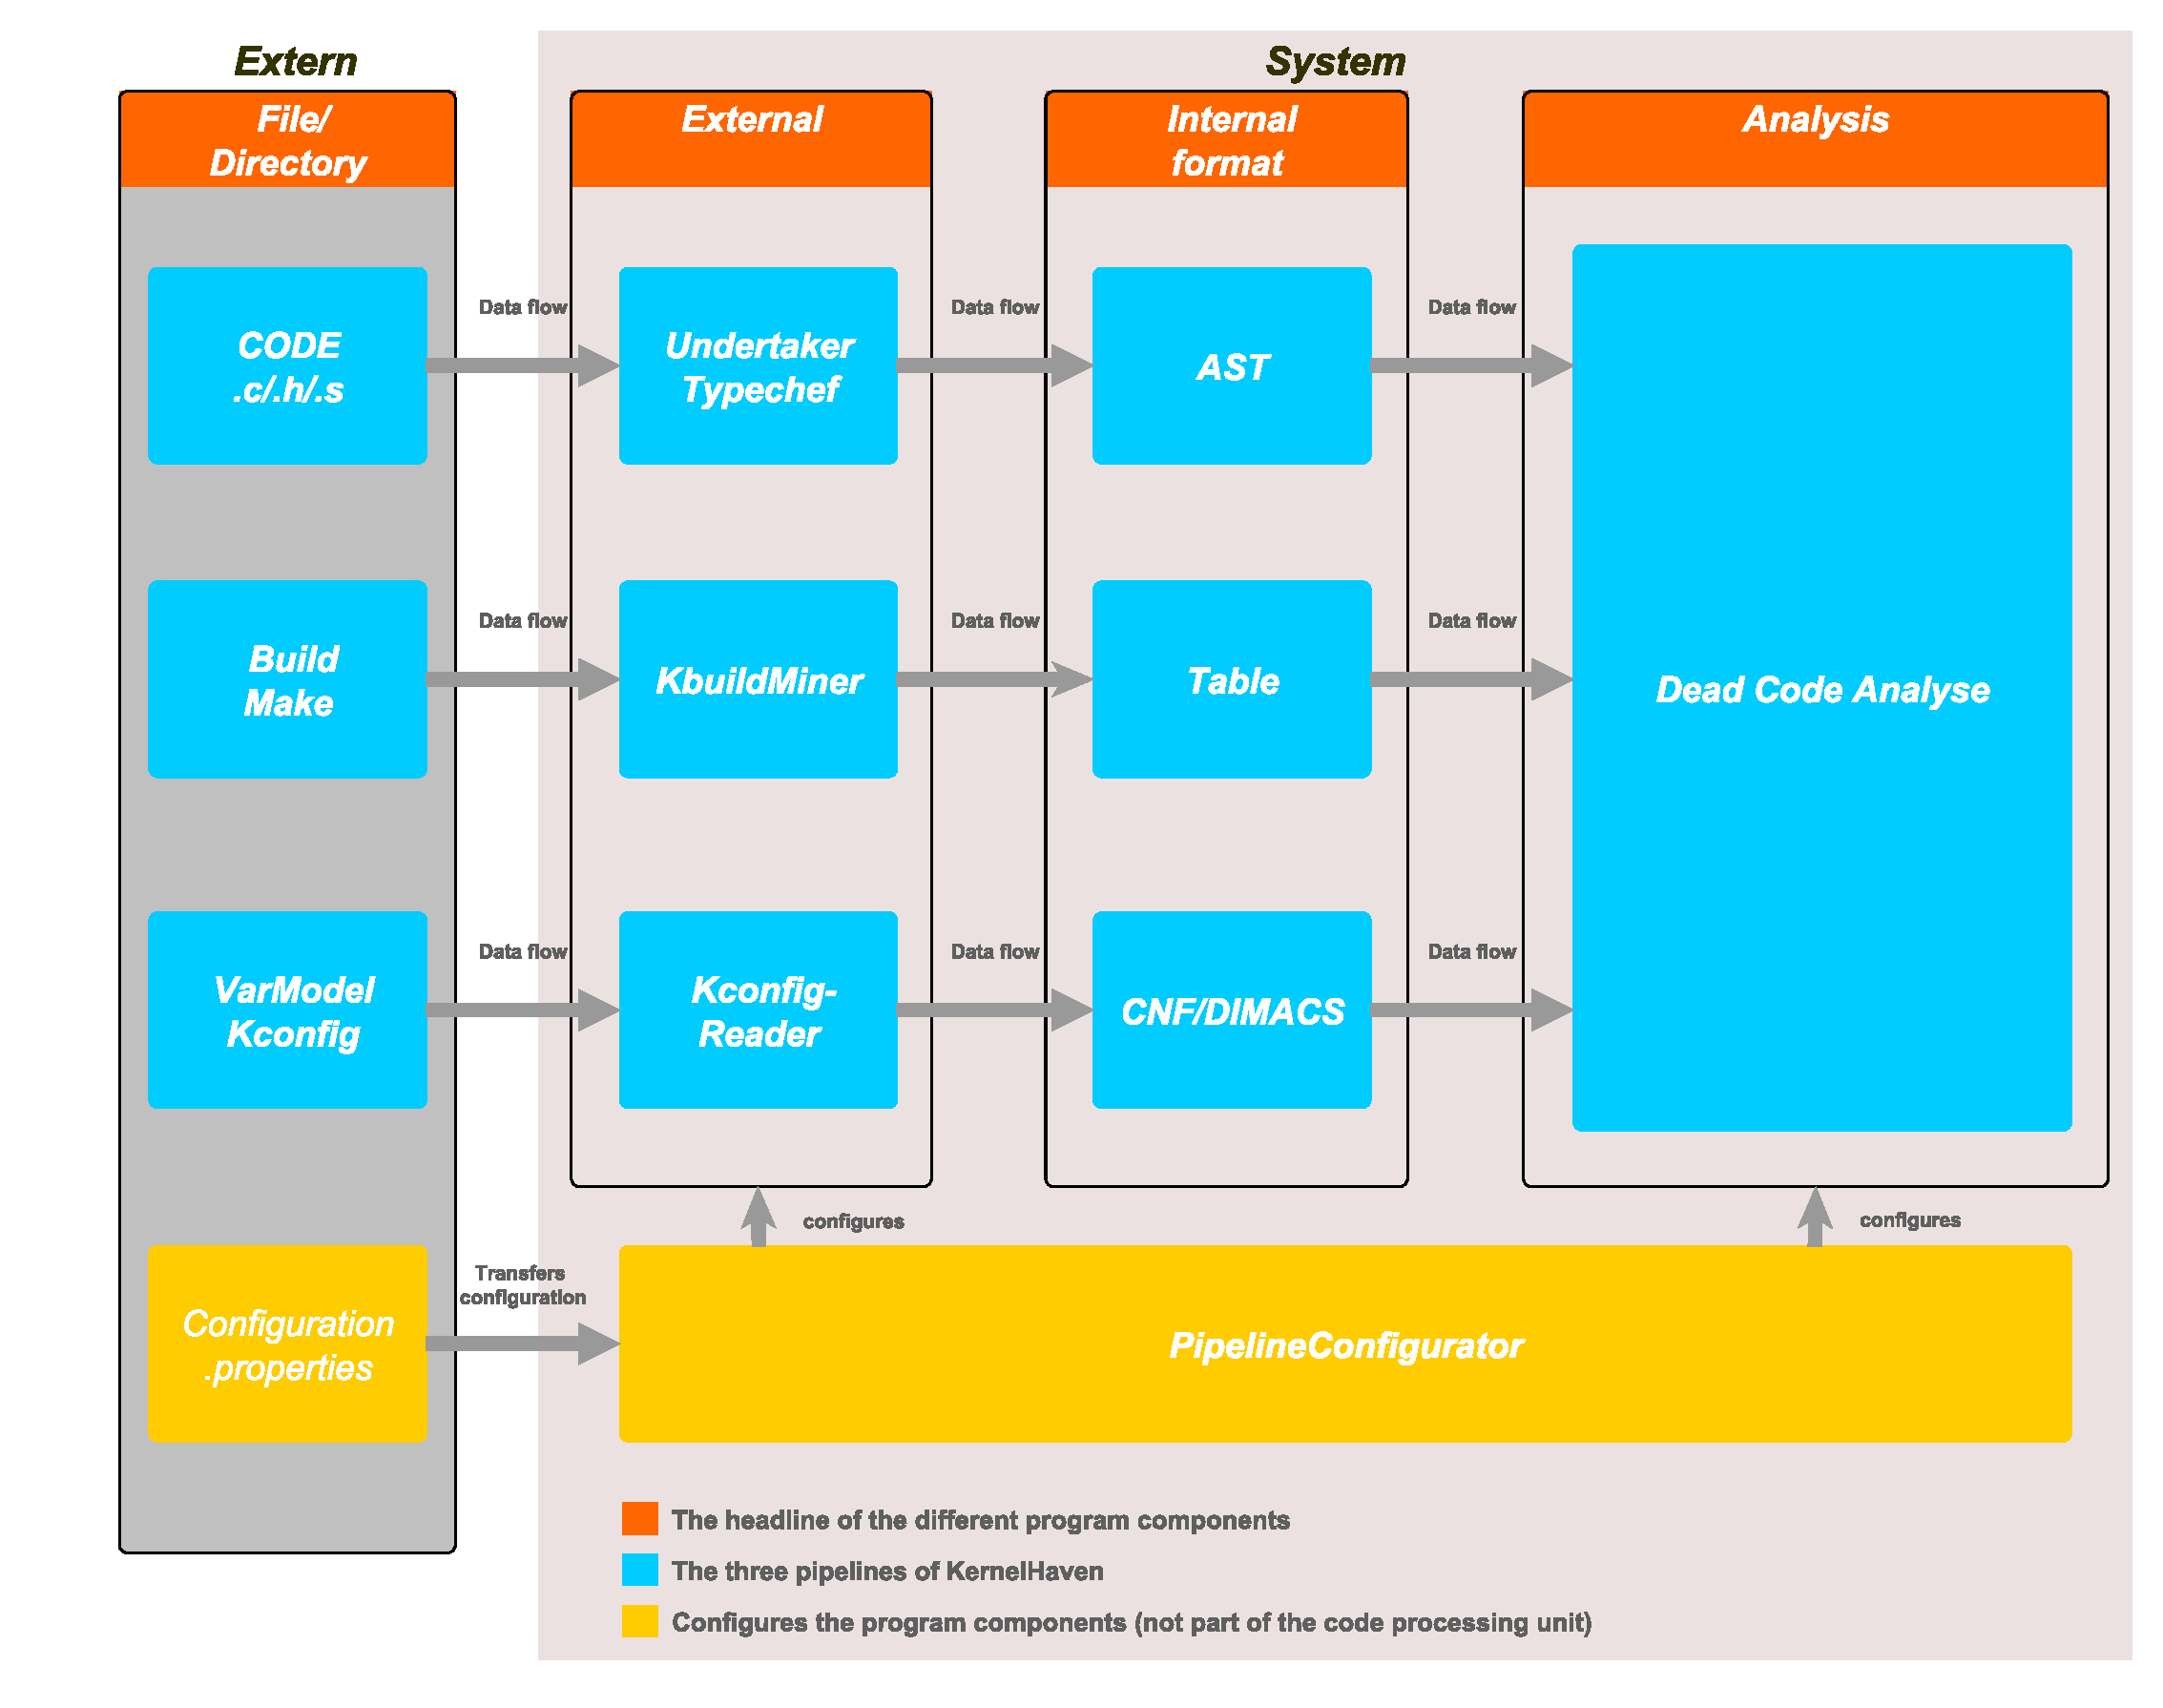
\includegraphics[width=1\textwidth]{Bilder/arch_simple.pdf}
  \end{minipage}
\end{figure}

%As the picture shows , the headline of the different program components is represented in red, whereas the actual program flow is represented in both blue and yellow, blue for the three pipelines that the program contains and yellow for the \texttt{configuration .properties} as well as the pipeline configurator which are not parts of the code processing unit but only responsible for configuring the system components.


%%%%%%%%%%%%%%%%%%%%%%%%%%%%%%%%%%%%%%%%%%%%%%%%%%%%%%%%%%%%%%%%%%%%%%%%%%%%%%%%%
% ***** 

\section{Configuration through a Properties-File} \label{properties}

The Properties-File follows the generic pattern of a java Properties-file. 
The properties described on the following pages are also included in the file \texttt{config\_template.properties} that is included in every release of KernelHaven. The collection of parameters only includes parameters that are integrated into the KernelHaven infrastructure. Any plugin might require more parameters for its execution. Please consult the documentation of the according plugin for more information (See \autoref{plugins}).

Some parameters include a \texttt{default:} value while others contain a \texttt{example:} value. The reason for this is that not all parameters have default values and while default-values also provide a good example of a valid value, an explicit example was needed for those parameters.

The description following \texttt{mandatory:}  reflects whether a parameter is optional or not. "yes" means that the parameter is required in every configuration. "no" without any additional information means that the parameter is optional in every configuration. There are some parameters with additional information for \texttt{mandatory} that explains under which circumstances the parameter becomes mandatory.

All parameters that have \texttt{default}-values are optional.

For boolean properties: Anything but "true" is read as "false"; the "true" is not case sensitive. If a boolean setting is missing and no default value is specified, then it is read as false.

\begin{table}[t] % unter die einl
    \caption{General Parameters} \label{tab:propfile}
    \begin{tabularx}{\textwidth}{|p{0.352\textwidth}|p{0.59\textwidth}|}\hline
        \textbf{Parameter} & \textbf{Description} \\ \hline \hline
        
        \texttt{resource\_dir} \newline example: \textcolor{blue}{/some/folder/tmp} \newline mandatory: yes  & The path where extractors can store their resources. The extractors create sub-folders in this called the same as their fully qualified class names (to prevent conflicts). This has to be always set to a valid directory with write and read access.\\ \hline
        
        \texttt{output\_dir} \newline example: \textcolor{blue}{/some/folder/output} \newline mandatory: yes & The path where the output files of the analysis will be stored. This has to be always set to a valid directory with write access. \\ \hline
        
        \texttt{plugins\_dir} \newline example: \textcolor{blue}{/some/folder/plugins} \newline mandatory: yes & The directory where plugins should be placed. All *.jar files in that directory will be loaded into the JVM. This means that 3rd party libraries which are required by plugins can also be included through this directory. This has to be always set to a valid directory with read access. \\ \hline
        
        \texttt{cache\_dir} \newline example: \textcolor{blue}{/some/folder/dir} \newline mandatory: no & This is the directory where the providers will write and read their cache. If \texttt{cache.read} or \texttt{cache.write} of a provider is set to true, then this has to be set to a valid directory with write and read access.\\ \hline
        
        \texttt{log.dir} \newline example: \textcolor{blue}{/some/folder/log} \newline mandatory: no  & This is the path where log files will be written. Needs to be defined if \texttt{log.file} is true. If required this has to be set to a valid directory with write access. \\ \hline
        
        \texttt{log.console} \newline default: \textcolor{blue}{true}  \newline mandatory: no & If set to true all logging sequences will be pushed to console, excluding huge third party outputs which will be trimmed to 500 characters. If a detailed output is needed refer to logging.file for a complete output. \\ \hline

        \texttt{log.file} \newline default: \textcolor{blue}{false}  &  If set to true all logging sequences will be pushed to a log file in the directory defined in \texttt{log.dir} setting.\\ \hline
        
        \texttt{log.error} \newline default:  \textcolor{blue}{true} & If set to false error log messages will be excluded from logging. \\ \hline
        
        \texttt{log.warning} \newline default: \textcolor{blue}{true} & If set to false warning log messages will be excluded from logging. \\ \hline
        
        \texttt{log.info} \newline default: \textcolor{blue}{true} & If set to false info log messages will be excluded from logging. \\ \hline
        
        \texttt{log.debug} \newline default: \textcolor{blue}{false} & If set to false debug log messages will be excluded from logging. \\ \hline
        
        \texttt{archive} \newline default: \textcolor{blue}{false} & Archives the the tool and its configuration including all artifacts and results. Alternative to setting the \texttt{$--$archive} flag on terminal. \\ \hline
        
        \texttt{archive.dir} \newline example: \textcolor{blue}{/some/dir} & Directory to write the archive of the current configuration and results to. \\ \hline
        
    \end{tabularx}
\end{table}

\begin{table}[t] % unter die einl
    \caption{Analysis Parameters} \label{tab:propfile}
    \begin{tabularx}{\textwidth}{|p{0.352\textwidth}|p{0.59\textwidth}|}\hline
    \textbf{Parameter} & \textbf{Description} \\ \hline \hline
    
    \texttt{analysis.class} \newline example: \textcolor{blue}{some.package.ClassName} \newline mandatory: yes & The fully qualified class name of the analysis that should be run. \\ \hline
    
    \end{tabularx}
\end{table}

\begin{table}[t] % unter die einl
    \caption{Common Extractor Parameters} \label{tab:propfile}
        \begin{tabularx}{\textwidth}{|p{0.352\textwidth}|p{0.59\textwidth}|}\hline
        \textbf{Parameter} & \textbf{Description} \\ \hline \hline
        
        \texttt{source\_tree} \newline example: \textcolor{blue}{/some/source/tree} \newline mandatory: depends on extractors & The path to the source tree that should be analyzed. \\ \hline
        
        \texttt{arch} \newline example: \textcolor{blue}{x86}  \newline mandatory: depends on extractors & The architecture  of the Linux kernel that should be analyzed. \\ \hline
    \end{tabularx}
\end{table}

\begin{table}[t] % unter die einl
    \caption{Parameters for Code Model} \label{tab:propfile}
    \begin{tabularx}{\textwidth}{|p{0.352\textwidth}|p{0.59\textwidth}|}\hline
    
        \textbf{Parameter} & \textbf{Description} \\ \hline \hline

        \texttt{code.provider.timeout} \newline default: \textcolor{blue}{0} & The maximum time the provider waits for the results of the extractor until an exception is thrown in milliseconds, 0 means no timeout used. \\ \hline    
        
        \texttt{code.provider.cache.write} \newline default: \textcolor{blue}{false} \newline mandatory: no & If set to true, then the code model provider will write its results to the cache directory.\\ \hline
         
        \texttt{code.provider.cache.read} \newline default: \textcolor{blue}{false}  \newline mandatory: no &  If set to true, then the code model provider is allowed to read the cache instead of starting the extractor. \\ \hline

        \texttt{code.extractor.class} \newline example: \textcolor{blue}{some.package.ClassName} \newline mandatory: no, but may be required by analysis & The fully qualified class name of the extractor for the code model. \\ \hline

        \texttt{code.extractor.files} \newline example: \textcolor{blue}{file1.c, dir/file2.c, dir/subdir/} \newline default: empty & Defines which files the code extractor should run on. Comma separated list of paths relative to the source tree. If directories are listed, then they are searched recursively for files that match the \texttt{code.extractor.file\_regex} pattern. Leave empty to specify the complete source tree. \\ \hline
        
        \texttt{code.extractor.file\_regex} \newline example: \textcolor{blue}{.*$\textbackslash$.(h|c|S)} \newline default: \textcolor{blue}{.*$\textbackslash$.c} & A Java regular expression defining which files are considered to be source files for parsing. \\ \hline
        
        \texttt{code.extractor.threads} \newline default: \textcolor{blue}{1} & The number of threads the code extractor should use. This many files are parsed in parallel. \\ \hline
        
    \end{tabularx}
\end{table}

\begin{table}[t] % unter die einl
    \caption{Parameters for Build Model} \label{tab:propfile}
    \begin{tabularx}{\textwidth}{|p{0.352\textwidth}|p{0.59\textwidth}|}\hline
        \textbf{Parameter} & \textbf{Description} \\ \hline \hline

        \texttt{build.provider.timeout}  \newline default: \textcolor{blue}{0} \newline mandatory: no  & The maximum time the provider waits for the results of the extractor until an exception is thrown in milliseconds. 0 means no timeout is used. \\ \hline

        \texttt{build.provider.cache.write} \newline default: \textcolor{blue}{false} \newline mandatory: no & If set to true, then the build model provider will write its result to the cache directory.\\ \hline
         
        \texttt{build.provider.cache.read} \newline default: \textcolor{blue}{false}  \newline mandatory: no &  If set to true, then the build model provider is allowed to read the cache instead of starting the extractor. \\ \hline
        
        \texttt{build.extractor.class} \newline example: \textcolor{blue}{some.package.ClassName}  \newline mandatory: no, but may be required by analysis & The fully qualified class name of the extractor for the build model. \\ \hline
    \end{tabularx}
\end{table}




\begin{table}[t] % unter die einl
    \caption{Parameters for Variability Model} \label{tab:propfile}
    \begin{tabularx}{\textwidth}{|p{0.432\textwidth}|p{0.51\textwidth}|}\hline
        \textbf{Parameter} & \textbf{Description} \\ \hline \hline
        
        \texttt{variability.provider.timeout} \newline default: \textcolor{blue}{0} \newline mandatory: no  & The maximum time the provider waits for the results of the extractor until an exception is thrown in milliseconds. 0 means no timeout is used. \\ \hline
        
        \texttt{variability.provider.cache.write} \newline default: \textcolor{blue}{false} \newline mandatory: no & If set to true, then the variability model provider will write its result to the cache directory. \\ \hline 
        
        \texttt{variability.provider.cache.read} \newline default: \textcolor{blue}{false} \newline mandatory: no & If set to true, then the variability model provider is allowed to read the cache instead of starting the extractor.\\ \hline
                
        \texttt{variability.extractor.class} \newline example: \textcolor{blue}{some.package.ClassName}  \newline mandatory: no, but may be required by analysis & The fully qualified class name of the extractor for the variability model. \\ \hline
        
        \texttt{variability.extractor.}\newline \texttt{find\_locations} \newline default: \textcolor{blue}{false}  & If set to true, the extractor will store source locations for each variable. Those locations represent occurrences of the variable in the files that kconfigreader used for generating the VariabilityMode. \\ \hline
     
    \end{tabularx}
\end{table}

\chapter{KernelHaven Plugins}\label{plugins}

%\section{Template}


%\textbf{Type:} BuildModel-Extractor / CodeModel-Extractor / VariabilityModel-Extractor / Analyis-Plugin

%\textbf{Class:} path.to.Class

%\textbf{License:} GPL / LGPL / ... / KernelHaven-License

%\textbf{Prerequisites:}

%What input is needed? Does other software need to be installed? Are there limitations (only working on linux-kernel etc.)?

%\textbf{Capabilities:}

%What are the possiblities and limitations of the tool? What aspects of the input are processed?

%\textbf{Additional Parameters:}

%Describe parameters that are needed in addition to the common parameters of the KernelHaven-Infrastructure in \autoref{properties}.

%\begin{table}[h!] % unter die einl
%    \begin{tabularx}{\textwidth}{|p{0.352\textwidth}|p{0.59\textwidth}|}\hline
%        \textbf{Parameter} & \textbf{Description} \\ \hline \hline
%        \texttt{parameter} \newline example: \textcolor{blue}{some.value}  \newline mandatory: yes, if PluginName is used &  \\ \hline
%        

%    \end{tabularx}
%\end{table}

\section{DeadCodeAnalysis (Part of DefaultAnalyses)}

\textbf{Type:}  Analyis-Plugin

\textbf{Class:} \texttt{de.uni\_hildesheim.sse.kernel\_haven.default\_analyses.DeadCodeAnalysis}

\textbf{License:} KernelHaven-License

\textbf{Prerequisites:}

Needs the three extractors for the variability model, build model and code model. Depends on CnfUtils.

\textbf{Capabilities:}

This is a simple implementation to detect dead code blocks. It considers file presence conditions and ifdef blocks.

\textbf{Additional Parameters:}

None.

\section{Missing Analysis  (Part of DefaultAnalyses)}

\textbf{Type:}  Analyis-Plugin

\textbf{Class:} \texttt{de.uni\_hildesheim.sse.kernel\_haven.dummy\_analysis.MissingAnalysis}

\textbf{License:} KernelHaven-License

\textbf{Prerequisites:}

Needs the three extractors for the variability model, build model and code model.

\textbf{Capabilities:}

This analysis uses the variability model and returns a file of all variables which are defined in the variability model but not used in the code model or build model, or a file of all variables which are used in the code model or build model but not defined in the variability model.

\textbf{Additional Parameters:}

\begin{table}[h!] % unter die einl
    \begin{tabularx}{\textwidth}{|p{0.352\textwidth}|p{0.59\textwidth}|}\hline
        \textbf{Parameter} & \textbf{Description} \\ \hline \hline
        
        \texttt{analysis.missing.type} \newline default: \textcolor{blue}{D}  \newline & This parameter is for choosing the missing analysis. The parameter \textcolor{blue}{D} is for the 'defined but not used' analysis. The parameter \textcolor{blue}{U} is for the 'used but not defined' analysis.  This is not case sensitive.\\ \hline
        
    \end{tabularx}
\end{table}


\section{KBuildMinerExtractor}

\textbf{Type:}
BuildModel-Extractor

\textbf{Class:} \texttt                             {de.uni\_hildesheim.sse.kernel\_haven.kbuildminer.KbuildMinerExtractorFactory}

\textbf{License:}
GPL-3.0 

KernelHaven-License would be possible with following restrictions:

The extractor contains kbuildminer.jar which is under GPL-3.0. We do not link against kbuildminer, so technically we are not infected by GPL. However a release under a license other than GPL-3.0 would require the removal of the contained kbuildminer.jar.

\textbf{Prerequisites:}

None.

\textbf{Capabilities:}

This extractor finds presence conditions of source files defined in Kbuild.

\textbf{Additional Parameters:}

\begin{table}[h!] % unter die einl
    \begin{tabularx}{\textwidth}{|p{0.352\textwidth}|p{0.59\textwidth}|}\hline
        \textbf{Parameter} & \textbf{Description} \\ \hline \hline
        
        \texttt{build.extractor.top\_folders} \newline example: \\ \textcolor{blue}{kernel,drivers,arch/x86}  \newline mandatory: no & List of top folders to analyze in the product line. If not supplied, then a default set for Linux is generated from the \texttt{arch} setting. \\ \hline
        
    \end{tabularx}
\end{table}


\section{KConfigReaderExtractor}

\textbf{Type:} VariabilityModel-Extractor

\textbf{Class:} \texttt{de.uni\_hildesheim.sse.kernel\_haven.kconfigreader.KconfigReaderExtractorFactory}


\textbf{License:} GPL-3.0 

KernelHaven-License would be possible with following restrictions:

The extractor contains kconfigreader.jar which is under GPL-3.0. We do not link against kconfigreader, so technically we are not infected by GPL. However a release under a license other than GPL-3.0 would require the removal of the contained kconfigreader.jar.

\textbf{Prerequisites:}

This extractor can only run on a Linux operating system. It also requires make and gcc (\texttt{\$ apt-get install  build-essential libelf-dev bc}).

\textbf{Capabilities:}

This extractor reads the Kconfig model. To do that, it has to modify the Linux source tree by calling \texttt{make allyesconfig prepare} on it. Be aware that this overrides any previously present \texttt{.config} file in the Linux source tree.

\textbf{Additional Parameters:}

None.

%\begin{table}[h!] % unter die einl
%    \begin{tabularx}{\textwidth}{|p{0.352\textwidth}|p{0.59\textwidth}|}\hline
%        \textbf{Parameter} & \textbf{Description} \\ \hline \hline
%        \texttt{parameter} \newline example: \textcolor{blue}{some.value}  \newline mandatory: yes, if PluginName is used &  \\ \hline
%        
%        \texttt{arch} \newline example: \textcolor{blue}{x86}  \newline mandatory: no, but may be required by some extractors & The architecture  of the Linux kernel that should be analyzed \\ \hline
%    \end{tabularx}
%\end{table}


\section{UndertakerExtractor}

\textbf{Type:} CodeModel-Extractor

\textbf{Class:} \texttt{de.uni\_hildesheim.sse.kernel\_haven.undertaker.UndertakerExtractorFactory}

\textbf{License:}

KernelHaven-License would be possible with following restrictions:

The extractor contains undertaker which is under GPL-3.0. We do not link against undertaker, so technically we are not infected by GPL. However a release under a license other than GPL-3.0 would require the removal of the contained undertaker.

\textbf{Prerequisites:}

This extractor can only run on a Linux operating system.

\textbf{Capabilities:}

This extractor finds \texttt{\#ifdef} blocks in source files.

\texttt{ExpressionFormatException}  is a common exception thrown by this extractor. This is the expected behaviour because ifdef-Blocks often contain non-boolean expressions while we only work with boolean expressions. This needs to be handled in any analysis using this extractor.

\textbf{Additional Parameters:}

\begin{table}[h!] % unter die einl
    \begin{tabularx}{\textwidth}{|p{0.352\textwidth}|p{0.59\textwidth}|}\hline
        \textbf{Parameter} & \textbf{Description} \\ \hline \hline
        
        \texttt{code.extractor.hang\_timeout} \newline default: \textcolor{blue}{20000} & Undertaker has a bug where it hangs forever on some few files of the Linux kernel. This setting defines a timeout in milliseconds until the undertaker executable is forcibly terminated. \\ \hline
        
    \end{tabularx}
\end{table}


%\section{TypeChefExtractor}

%\textbf{Type:} CodeModel-Extractor 

%\textbf{Class:} \texttt{de.uni\_hildesheim.sse.kernel\_haven.typechef.CLASS\_HERE}
%\todo{add the class name for TypeChef}

%\textbf{License:} GPL / LGPL / ... / KernelHaven-License

%\textbf{Prerequisites:}

%What input is needed? Does other software need to be installed? Are there limitations (only working on linux-kernel etc.)?

%\textbf{Capabilities:}

%What are the possiblities and limitations of the tool? What aspects of the input are processed?

%\textbf{Additional Parameters:}

%Describe parameters that are needed in addition to the common parameters of the KernelHaven-Infrastructure in \autoref{properties}.

%\begin{table}[h!] % unter die einl
%    \begin{tabularx}{\textwidth}{|p{0.352\textwidth}|p{0.59\textwidth}|}\hline
%        \textbf{Parameter} & \textbf{Description} \\ \hline \hline
%        \texttt{parameter} \newline example: \textcolor{blue}{some.value}  \newline mandatory: yes, if PluginName is used &  \\ \hline
%        
%        \texttt{arch} \newline example: \textcolor{blue}{x86}  \newline mandatory: no, but may be required by some extractors & The architecture  of the Linux kernel that should be analyzed \\ \hline
%    \end{tabularx}
%\end{table}


\chapter{Examples}

\section{DummyAnalysis}

The execution environment in this example is a machine running Ubuntu 16.04 with all of the packages listed in \autoref{setup} installed. 

First, the entire contents of the binary-release of KernelHaven need to be extracted. In our case, we choose to extract the contents of the zip-archive (binary-release) to a directory our desktop. You may however choose any other directory with read/write access to reproduce this on your own machine.

Now \texttt{kernelhaven.jar}, \texttt{dummy\_analysis.properties}, \texttt{config\_template.properties} and the folder  \texttt{plugins} with all of the plugins contained in the release are present in the directory that we just created.

Additionally, we create the folders "cache", "output" and "res" inside of the same directory that already contains \texttt{kernelhaven.jar}.

On the desktop we have a folder \texttt{linux-releases} containing the linux kernel  linux-4.4.56 as shown in \autoref{fig:DummyAnalysisFolderStructure}. You can use any other version of the linux kernel but will have to adjust the parameter \texttt{source\_tree} in \texttt{dummy\_analysis.properties} accordingly.

\begin{figure}[h!] 
  \centering
  \begin{minipage}[b]{1\textwidth} 
    \caption{Folder Strucure}\label{fig:DummyAnalysisFolderStructure}
    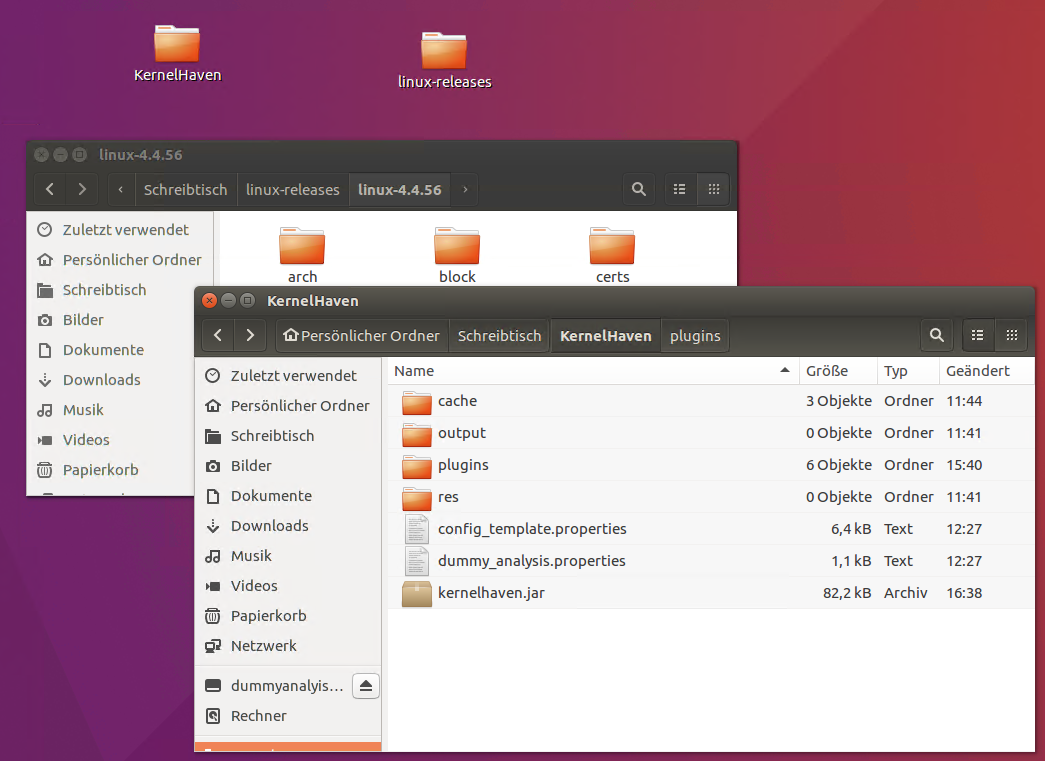
\includegraphics[width=1\textwidth]{Bilder/DummyAnalysisFolderStructure.png}
  \end{minipage}
\end{figure}


We will use the configuration \texttt{dummy\_analysis.properties} that is contained in every release. This configuration can be used to confirm that the KernelHaven-infrastucture is working.  \texttt{dummy\_analysis.properties} includes every relevant folder setting as relative path. If you choose to setup your folders in a different way, you might need to use absolute paths instead for those parameters.

Now we open the console and change to the directory in which \texttt{kernelhaven.jar} is contained. 

\begin{lstlisting} [language=console]
    $ cd ~/Desktop/KernelHaven/
\end{lstlisting}


Because \texttt{kernelhaven.jar} is in the same the directory as \texttt{dummy\_analysis.properties} we can execute KernelHaven by only passing a relative path as parameter.

\begin{lstlisting} [language=console]
    $ java -jar kernelhaven.jar dummy_analysis.properties
\end{lstlisting}

After running the command, the console shows the output of the KernelHaven-Execution.


\end{spacing}


\end{document}